\documentclass[a4paper]{article}
\usepackage[margin=1.5cm]{geometry}

%Links
\usepackage[colorlinks = true,
            linkcolor = blue,
            urlcolor  = blue,
            citecolor = blue,
            anchorcolor = blue]{hyperref}

%Simbolos matemáticos
\usepackage{amsmath}
\usepackage{amssymb}

%Enumeracion
\usepackage{enumitem}

%Multicolumna
\usepackage{multicol}

%Graficos
\usepackage{graphicx}

%Páginas sin numeración
\pagestyle{empty}

%Interlineado
\renewcommand{\baselinestretch}{1.5}

%Arreglar comillas
\usepackage [autostyle]{csquotes}
\MakeOuterQuote{"}

% Formato de enumitem de incisos
\setlist[enumerate,2]{label=(\alph*)}

% Define a new environment that combines enumerate with multicols
\NewDocumentEnvironment{enumcols}{O{1}}
{
  \ifnum#1>1 \begin{multicols}{#1} \fi
  \begin{enumerate}
}
{
  \end{enumerate}
  \ifnum#1>1 \end{multicols} \fi
}

%Macros
\newcommand{\Item}{\item[\stepcounter{enumii}$\blacktriangleright$\textbf{(\alph{enumii})}]} %Negrita en algunos items
\newcommand{\answer}{\item[**]} % Respuesta
\newcommand{\exercise}{\item} % Ejercicio
\newcommand{\SEL}[1]{\left\{\begin{matrix} #1 \end{matrix}\right.} %Sistema de ecuaciones lineales
\newcommand{\AMat}[2]{\left(\begin{array}{@{}*{#1}{c}|c@{}} #2 \end{array}\right)} % Matriz ampliada
\newcommand{\Mat}[1]{\begin{pmatrix} #1 \end{pmatrix}}
\newcommand{\Det}[1]{\begin{vmatrix} #1 \end{vmatrix}}
\newcommand{\f}[2]{\displaystyle\frac{#1}{#2}} % Fracción grande
\newcommand{\conj}[1]{\overline{#1}} % Conjugado de complejo
\newcommand{\cis}[1]{\left[\cos\left({#1}\right)+i\sin\left({#1}\right)\right]} %Forma trigonométrica de complejo
\newcommand{\img}[2]{ \begin{minipage}[t]{\linewidth} \raisebox{-\height}{\includegraphics[width=#1]{#2}} \end{minipage} } % Imagen en inciso
\newcommand{\vect}[1]{\overrightarrow{#1}} %Vector con flecha amplia
\newcommand{\degs}{^{\circ}} % Grados
\newcommand{\R}{\mathbb{R}} % Conjunto de los reales
\newcommand{\C}{\mathbb{C}} % Conjunto de los complejos
\newcommand{\Cmat}[2]{\mathbb{C}^{{#1} \hspace{-0.2mm}\times \hspace{-0.2mm} {#2}}} % Matrices complejas
\newcommand{\Z}{\mathbb{Z}} % Conjunto de los enteros
\newcommand{\Q}{\mathbb{Q}} % Conjunto de los racionales
\newcommand{\ivec}{\check{\imath}} % i vector
\newcommand{\jvec}{\check{\jmath}} % j vector
\newcommand{\kvec}{\check{k}} % k vector


\begin{document}

\noindent \hrulefill 
\vspace{-7pt}
\begin{center} 
	\textbf{ Práctica 7: Rectas y Planos } \\
	Comisión: Rodrigo Cossio-Pérez y Gabriel Romero
\end{center}
\vspace{-10pt}
\hrulefill


\begin{enumerate}

	\exercise Hallar una recta del plano que cumpla con las siguientes condiciones. Dar una ecuación implícita o general, explícita, paramétrica vectorial, paramétrica cartesiana y simétrica. Indicar si la recta hallada es única.
	\begin{enumcols}
		
		\item Pasa por el punto $P(-3,1)$ y es paralela al vector $\vec{d}=(2,-1)$
		\answer La recta es única. \\ Algunas ecuaciones: $(x,y)=(-3,1)+k(2,-1)$. \\ $\SEL{ x=-3+2k \\ y=1-k \hfill }$ \\ $\f{x+3}{2}=\f{y-1}{-1}$.

		\item Pasa por el punto $P(1,2)$ y es paralela al vector $\vect{AB}$ con $A(2,-5)$ y $B(4,-5)$
		\answer La recta es única. Se utiliza $\vect{AB}=(2,0)$ como director. \\ $(x,y)=(1,2)+k(2,0)$. \\ $\SEL{ x=1+2k \\ y=2 \hfill }$ \\ $y=2$.\\ $y-2=0$. \\ No existe simétrica.

		\item Es coincidente con la recta $L: 2x-y+8=0$
		\answer La recta es única. $4x-2y+16=0$. $y=2x+8$. $(x,y)=(0,8)+k(1,2)$. \\ $\SEL{ x=k \hfill \\ y=8+2k }$ \\ $x=\f{y-8}{2}}$.

		\item Pasa por los puntos $P(-3,0)$ y $Q(-3,3)$
		\answer La recta es única. Se utiliza $\vect{PQ}=(0,3)$ como director. \\ $(x,y)=(-3,0)+k(0,3)$  \\ $\SEL{ x=-3 \\ y=3k }$ \\ $x=-3$. \\ $x+3=0$. \\ No existe simétrica.

		\item Pasa por el punto $P(1,4)$ y pendiente $-\f{1}{2}$
		\answer La recta es única. $y=-\f{1}{2}x+\f{9}{2}$. $(x,y)=(1,4)+k(2,-1)$. \\ $\SEL{ x=1+2k \\ y=4-k }$ \\ $\f{x-1}{2}=\f{y-4}{-1}$.

		\item Pasa por el origen y es perpendicular al vector $\vec{n}=(2,3)$
		\answer La recta es única. Se utiliza $\vec{d}=(-3,2)$ como director ya que $\vec{n} \perp \vec{d}$. \\ $(x,y)=k(-3,2)$. \\ $\SEL{ x=-3k \\ y=2k }$ \\ $\f{x}{-3}=\f{y}{2}$.

		\item Pasa por el punto $P(1,2)$ y es perpendicular al eje de abscisas (eje $x$)
		\answer La recta es única. Se utiliza $\jvec$ como director ya que $\jvec \perp \ivec$. \\ $(x,y)=(1,2)+k(0,1)$. \\ $\SEL{ x=1 \hfill\\ y=2+k }$ \\ $x=1$. \\ $x-1=0$. \\ No existe simétrica.

		\item Tiene a -4 como absisa al origen y 3 como ordenada al origen
		\answer La recta es única. De los puntos $A(-4,0)$ y $B(0,3)$ se obtiene el vector director $\vect{AB}=(4,3)$. \\ $(x,y)=(0,3)+k(4,3)$. \\ $\SEL{ x=4k \hfill \\ y=3+3k }$ \\ $\f{x}{4}=\f{y-3}{3}$.

		\item Pasa por los puntos $P(-3,1)$, $Q(1,3)$, $R(3,-3)$
		\answer No existe una recta que cumpla con las condiciones ya que los puntos no están alineados. Se puede ver porque $\vect{PQ} \nparallel\vect{QR}$

		\item Corta al eje de ordenadas en el punto $M(0,2)$
		\answer La recta NO es única, la misma responde a la ecuación $y=mx+2$ o $(x,y)=(0,2)+k(a,b)$. Por ejemplo, se elije $m=1$ y se obtiene la recta $y=x+2$.

		\item Forma un ángulo de $30\degs$ con el eje de abscisas (eje $x$).
		\answer La recta NO es única. Se obtiene el vector unitario $\hat{d}=(\cos 30\degs, \sin 30\degs)=\left(\f{\sqrt{3}}{2},\f{1}{2}\right)$ como director. Se puede elegir cualquier punto para definir la recta. Por ejemplo, con $P(1,3)$ y se obtiene la recta $(x,y)=(1,3)+k\left(\f{\sqrt{3}}{2},\f{1}{2}\right)$.

		\item Pasa por el punto $P(3,-2)$ y es normal a $\vec{n}$, donde $\vec{n}$ es un vector con ángulo $\f{\pi}{4}$ con respecto al eje de ordenadas.
		\answer $\vec{n}$ puede ser $\vect{n_1}=(\cos 45\degs, \sin 45\degs)=\left(\f{\sqrt{2}}{2},\f{\sqrt{2}}{2}\right)$ o $\vect{n_2}=(\cos 135\degs, \sin 135\degs)=\left(-\f{\sqrt{2}}{2},\f{\sqrt{2}}{2}\right)$. Por lo que la recta no es única. Las opciones son: $(x,y)=(3,-2)+k\left(\f{\sqrt{2}}{2},\f{\sqrt{2}}{2}\right)$ o $(x,y)=(3,-2)+t\left(-\f{\sqrt{2}}{2},\f{\sqrt{2}}{2}\right)$.

	\end{enumcols}


	\exercise Analizar las posiciones relativas de las rectas del plano. Es decir, analizar si son paralelas, coincidentes, perpendiculares o incidentes. Calcular la intersección entre las rectas.
	\begin{enumcols}
		
		\item $s: 2x+y-1=0$ ~~y~~ $r:\SEL{x=1+2t \\ y=3-t}$
		\answer $s \parallel r$. $s \cap r=\emptyset$.  Resolución por \href{https://youtu.be/cHsXMw3V4mQ}{Elena Virseda}

		\item $r:\SEL{x=-3+2t \\ 4-t}$ ~~y~~ $s:\f{x+6}{-4}=\f{y-1}{2}$.
		\answer $r \parallel s$. $r \cap s=\emptyset$. Resolución por \href{https://youtu.be/MPUh70MKVUY}{Matemáticas y Física con Pablo}

		\item $r_1: 2x-4y=2$ ~~y~~ $r_2: x+y=0$.
		\answer $r_1$ y $r_2$ son incidentes no-perpendiculares ya que se intersectan en un punto y sus normales no son perpendiculares: $(2,-4) \not\perp (1,1)$. La intersección es $r_1 \cap r_2=\left\{ \left(\f{1}{3},-\f{1}{3}\right)\right\}$. \href{https://youtu.be/LgIU8pd8DeM?t=97}{Matemáticas con Huais}

		\item $r_1: x+3y=7$ ~~y~~ $r_2: (x,y)=(4,1)+\alpha (-6,2)$ con $\alpha \in\R$.
		\answer $r_1$ y $r_2$ son coincidentes. La intersección es $r_1 \cap r_2=r_1=r_2$. \href{https://youtu.be/LgIU8pd8DeM?t=884}{Matemáticas con Huais}

		\item $r: 2x-y-3=0$ ~~y~~ $s: (x,y)=(-1,0)+ k (-6,3)$ con $k\in\R$.
		\answer Reemplazamos $\SEL{x=-1-6k \\ y=3k \hfill}$ en $2x-y-3=0$ y obtenemos $k=-\f{1}{3}$. Por lo tanto, $r \cap s=\left\{ \left(1,-1\right)\right\}$. Además $\vect{n_r}=(2,-1)$ es paralela a $\vect{d_s}=(-6,3)$, por lo que $r \perp s$.

		\item $r: y=-\f{1}{2}x+\f{3}{2}$ ~~y~~ $s: \f{1}{4}x+\f{3}{4}y-3=0$.

		\item $r: (x,y)=(4,2-3k)$ ~~y~~ $s: (x,y)=(2-4h,-3)$ con $k,h\in\R$.

		\item $r: (x,y)=k(3,-2)+(10,5)$ con $k\in\R$ ~~y~~ $s: 2x+3y-35=0$.

	\end{enumcols}

	
	\exercise Graficar los siguientes lugares geométricos relacionados a rectas.
	\begin{enumcols}[2]

		\item $4x+3y > 4$

		\item $4x+3y \neq 4$

		\item $2x-y \leq 6$

		\item $2x-y < 6$

		\item $(x,y)=k(1,2)+(-2,3)$ con $k\in[0,+\infty)$
		\answer ~\\[-10pt] 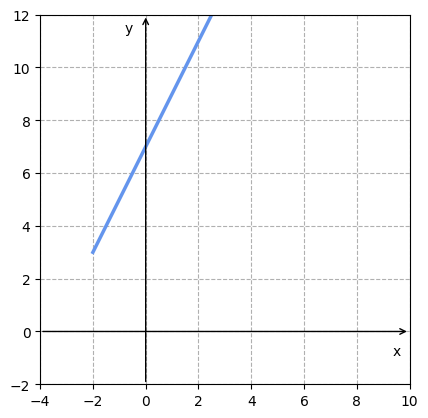
\includegraphics[width=55mm]{plots/plot1.png}

		\item $(x,y)=\lambda(1,2)+(0,3)$ con $\lambda\in\mathbb{Z}$

		\item $(x,y)=k(1,2)+(-1,3)$ con $k\in[-1,1]$

		\item $y=mx+2$ con $m\in[0,1)$

		\item $y=2x+b$ con $b\in[-2,1]$

		\item $R=\{(x,y) \in \R^2 ~|~ -x+y-5=0 ~\land~ 2x+y-17=0 \}$

		\item $S=\{(x,y) \in \R^2 ~|~ -x+y-5=0 ~\lor~ 2x+y-17=0 \}$

		\item $\SEL{-x+y-5=0 \\ 2x+y-17=0 \\ x+2y-10=0 }$

		\item $\SEL{-x+y-5=0 \\ 2x+y-17=0 \\ x+2y-17=0 \\ 3x+3y-34=0 }$
	
	\end{enumcols}


	\exercise Resolver los siguientes problemas integradores sobre la geometría en el plano.
	\begin{enumcols}
		
		\item Calcular la distancia entre el origen de coordenadas y la recta $r: 3x+4y -24=0$.

		\item Calcular la distancia entre el punto $(-1,7)$ y la recta $r: x-3y -10=0$.

		\item Encontrar un punto que equidiste de las rectas $r: x+2y-3=0$ y $s: -x-2y+4=0$ y otro que equidiste de las rectas $r$ y $t: 2x-y+1=0$.

		\item Calcular la distancia entre la recta que pasa por (1,-4) de pendiente -2 y la recta $r: 2x+y-6=0$.

		\item Calcular la distancia entre las rectas $r: (x,y)=t(4,4)+(2,-5)$ y $s: (x,y)=k(1,1)+(0,-9)$

		\item Calcular la proyección ortogonal del punto $P(3,-1)$ sobre la recta $r: -x-y-12=0$.

		\item Calcular la proyección ortogonal del punto $P(-2,2)$ sobre la recta $r: -5x+y-1=0$ y el punto simétrico $P'$.

		\item Hallar el valor de $a\in\R$ para que el ángulo entre $r_1: ax+3y=0$ ~y~ $r_2:\SEL{ x=4+\lambda \\ 1-2\lambda }$ sea de $30\degs$. 

	\end{enumcols}


	\exercise Hallar una recta del espacio que cumpla con las siguientes condiciones. Dar una ecuación paramétrica vectorial, paramétrica cartesiana y simétrica. Indicar si la recta hallada es única.
	\begin{enumcols}

		\item Pasa por los puntos $A(2,-3,1)$ y $B(-3,5,0)$.

		\item Es paralela al vector $(2,5,-2)$ y contiene al punto $P(4,-5,0)$.

		\item Incluye al punto $P(4,-5,0)$ y es perpendicular al vector $(2,5,-2)$.

		\item Es perpendicular a los vectores $(-2,0,0)$ y $(0,0,-6)$ y pasa por el punto $P(3,3,0)$

		\item Es paralela a $r: (x,y,z)=(2,4,-1)+t(-6,0,2)$ y pasa por $P(4,1,5)$.

		\item Es perpendicular a $r: (x,y,z)=(2,4,-1)+t(-6,0,2)$ y contiene a $P(4,1,5)$.

		\item Pasa por el punto $P(3,3,0)$ y es paralela a la recta $r: \SEL{y=z\\x=0}$

		\item Es perpendicular a $\pi: x+y+z-3=0$

		\item Es perpendicular a $\pi: 3x-2y+z=5$ y incluye a $P(4,1,5)$

		\item Es paralela a $\pi: 3x-2y+z=5$ y pasa por $P(4,1,5)$

		\item Es perpendicular a $r_1: \f{x+2}{2}=-y+3=\f{z+2}{5}$ y a $r_2: x-3=\f{2y-7}{2}=\f{z-3}{3}$ y contiene al punto $P(3,-3,4)$
		\answer $r: (x,y,z)=(3,-3,4)+t(-8,-1,3)$. \\ $r: \SEL{x=3-8y\\y=-3-t\\z=4+3t}$ \\ $r: \f{x-3}{-8}=\f{y+3}{-1}=\f{z-4}{3}$. \\ La recta es única. Resolución por \href{https://youtu.be/KebOzsUUmq4?t=458}{Mate316}.

		\item Pasa por el origen de coordenadas, es perpendicular a $r: (x,y,z)=(1,4,1)+t(3,-5,0)$ y no incluye a $P(0,0,3)$

		\item Está contenida en el plano $\pi: 2x-3y+2z=6$ y es perpendicular a la recta $r: (x,y,z)=(2,-9,7)+t(1,-1,1)$.

		\item Es paralela a los planos $\pi_1: 2x-3y+5z=2$ y $\pi_2: -x+3y+2z=1$ e incluye al punto $P(2,1,0)$.

	\end{enumcols}


	\exercise Hallar un plano que cumpla con las siguientes condiciones. Dar una ecuación implícita o general, explícita, paramétrica vectorial y paramétrica cartesiana. Indicar si el plano hallado es única.
	\begin{enumcols}

		\item  Pasa por el punto $P(2,2,2)$ y es perpendicular al vector $(3,-1,-2)$.

		\item  Es paralelo a los vectores $(2,0,2)$ y $(0,3,0)$ y pasa por el punto $P(1,2,0)$.

		\item  Pasa por los puntos $A(-1,1,1)$, $B(1,0,2)$ y $C(0,2,-2)$.

		\item  Es perpendicular al vector $(-2,0,1)$.

		\item  Es paralelo al vector $(2,-1,4)$ y pasa por el punto $P(3,3,1)$.

		\item  Pasa por los puntos $P(4,0,5)$ y $Q(-1,-1,0)$.

		\item  Pasa por los puntos $A(0,1,1)$, $B(1,3,2)$, $C(0,2,-4)$ y $D(1,7,5)$.

		\item  Pasa por los puntos $P(3,-2,0)$ y $Q(1,-1,1)$ y es paralelo al vector $(1,2,2)$.

		\item  Pasa por los puntos $P(3,-2,0)$ y $Q(1,-1,1)$ y es paralelo al vector $(1,2,2)$.

		\item  Es paralelo al plano $\pi: 2x-3y+2z=6$ y pasa por el punto $P(2,1,0)$.

		\item  Es paralelo a las rectas $r_1: (x,y,z)=(1,4,0)+t(5,5,-3)$ y $r_2: (x,y,z)=(-10,2,7)+t(4,0,3)$ y contiene al punto $P(2,2,2)$.

		\item  Es perpendicular a la recta $r: (x,y,z)=(2,-9,7)+t(1,-1,1)$ y pasa por el punto $P(3,1,-3)$.

		\item  Contiene a la recta $r: (x,y,z)=(5,1,0)+t(1,-3,1)$.

		\item Es perpendicular a los planos $\pi_1: 2x-3y+5z=2$ y $\pi_2: -x+3y+2z=1$ e incluye al punto $P(5,1,0)$.

		\item Es perpendicular al planos $\pi: 3x-2y+z=5$ y pasa por $P(4,1,5)$.

		\item  Contiene a la recta $r: (x,y,z)=(2,1,2)+t(0,4,1)$ y al punto $P(1,2,3)$

		\item  Contiene a las rectas $r_1: (x,y,z)=(13,-2,0)+t(-6,0,2)$ y $r_2: (x,y,z)=(-14,-8,16)+t(5,2,-4)$.

	\end{enumcols}


	\exercise Calcular la intersección de las siguientes rectas y/o planos.
	\begin{enumcols}

		\item $r_1: (x,y,z)=(13,-2,0)+t(-6,0,2)$ y $r_2: (x,y,z)=(-14,-8,16)+t(5,2,-4)$

		\item $r_1: (x,y,z)=(1,1,1)+t(1,2,3)$ y $r_2: (x,y,z)=(2,1,0)+t(3,8,13)$
		\answer $r_1 \cap r_2 = \{(5,9,13)\}$. Resolución por \href{https://youtu.be/KebOzsUUmq4?t=2304}{Mate316}.

		\item $r_1: (x,y,z)=(5,4,-1)+t(-6,0,2)$ y $r_2: (x,y,z)=(2,2,-1)+t(-3,2,1)$
		\item $r_1: (x,y,z)=(4,0,2)+t(2,4,6)$ y $r_2: (x,y,z)=(9,10,15)+t(3,6,9)$
		\item $\pi_1: 2x-3y+5z=2$ y $\pi_2: -x+3y+2z=1$.
		\item $\pi_1: 2x-4y+8z=3$ y $\pi_2: 3x-6y+12z=2$.
		\item $\pi_1: 2x-4y+8z=3$ y $\pi_2: 6x-12y+24z=9$.
		\item $r_1: (x,y,z)=(4,0,2)+t(2,4,6)$ y $\pi_2: 6x-12y+24z=9$
		\item $\pi_1: 2x-4y+8z=3$ y $r_2: (x,y,z)=(2,2,-1)+t(-3,2,1)$

	\end{enumcols}


	\exercise Resolver los siguientes problemas integradores sobre la geometría en el plano.
	\begin{enumcols}
		
		\item Dados los puntos $A(3,1,1)$ y $B(3,-2,4)$, y la recta $L: (x,y,z)=(1,-1,1)+t(1,1,0)$. Hallar un punto $C\in L$ tal que el ángulo entre $\vect{AB}$ y $\vect{AC}$ sea $60\degs$.
		
		\item Dadas las rectas $L_1$

	\end{enumcols}


\end{enumerate}

\end{document}